\documentclass[aspectratio=169,12pt]{beamer}
% Original "Evidence Ledger" theme for Measured Trust.
\usepackage[T1]{fontenc}
\usepackage[scaled=0.95]{helvet}
\renewcommand{\familydefault}{\sfdefault}
\usepackage{booktabs}
\usepackage{graphicx}
\usepackage{listings}
\usepackage{tikz}
\usepackage{xcolor}
\usepackage{ragged2e}

\definecolor{SignalTeal}{HTML}{0F766E}
\definecolor{EvidenceAmber}{HTML}{D97706}
\definecolor{ResolverViolet}{HTML}{6D28D9}
\definecolor{MidnightInk}{HTML}{0F172A}
\definecolor{Slate}{HTML}{475569}
\definecolor{WarmPaper}{HTML}{FCFAF5}
\definecolor{Mist}{HTML}{E7EEF0}
\definecolor{AuditRed}{HTML}{B42318}
\definecolor{VerifiedGreen}{HTML}{15803D}
\definecolor{CivicBlue}{HTML}{1D4ED8}

\setbeamercolor{background canvas}{bg=WarmPaper}
\setbeamercolor{normal text}{fg=MidnightInk,bg=WarmPaper}
\setbeamercolor{frametitle}{fg=MidnightInk,bg=WarmPaper}
\setbeamercolor{footline}{fg=Slate,bg=WarmPaper}
\setbeamercolor{structure}{fg=SignalTeal}
\setbeamerfont{normal text}{size=\fontsize{17}{21}}
\setbeamerfont{frametitle}{size=\fontsize{22}{25},series=\bfseries}
\setbeamerfont{footline}{size=\fontsize{8.5}{10}}
\setbeamertemplate{navigation symbols}{}
\setbeamersize{text margin left=0.72cm,text margin right=0.72cm}
\setlength{\parskip}{0.45em}
\raggedright

\setbeamertemplate{frametitle}{%
  \nointerlineskip
  \vspace{0.50cm}%
  \hbox{%
    \color{SignalTeal}\rule[-0.08cm]{0.10cm}{0.88cm}%
    \hspace{0.23cm}%
    \begin{minipage}[b]{0.90\paperwidth}%
      \raggedright\usebeamerfont{frametitle}\insertframetitle
    \end{minipage}%
  }%
  \vspace{0.12cm}%
}

\setbeamertemplate{footline}{%
  \leavevmode
  \hbox{%
    \begin{beamercolorbox}[wd=0.82\paperwidth,ht=0.38cm,dp=0.16cm,leftskip=0.72cm]{footline}%
      MEASURED TRUST \hspace{0.18cm}\textcolor{Mist}{|}\hspace{0.18cm} synthetic proof case
    \end{beamercolorbox}%
    \begin{beamercolorbox}[wd=0.18\paperwidth,ht=0.38cm,dp=0.16cm,rightskip=0.72cm plus1fil]{footline}%
      \hfill\insertframenumber/\inserttotalframenumber
    \end{beamercolorbox}%
  }%
}

\newcommand{\source}[1]{\vfill{\fontsize{8.5}{10}\selectfont\color{Slate}#1}}
\newcommand{\eyebrow}[1]{{\fontsize{10}{12}\selectfont\bfseries\color{SignalTeal}\MakeUppercase{#1}}}
\newcommand{\bigmetric}[2]{%
  {\fontsize{35}{37}\selectfont\bfseries\color{#1}#2}%
}
\newcommand{\ledgerbox}[3]{%
  \colorbox{#1!8}{%
    \begin{minipage}[t][2.35cm][c]{\dimexpr\linewidth-2\fboxsep\relax}
      \centering
      {\fontsize{12}{14}\selectfont\bfseries\color{#1}\MakeUppercase{#2}}\par
      \vspace{0.12cm}
      {\fontsize{15}{18}\selectfont\bfseries\color{MidnightInk}#3}
    \end{minipage}%
  }%
}

\lstdefinestyle{ledgercode}{
  basicstyle=\ttfamily\fontsize{11}{13}\selectfont,
  keywordstyle=\color{ResolverViolet}\bfseries,
  stringstyle=\color{SignalTeal},
  commentstyle=\color{Slate},
  backgroundcolor=\color{Mist!55},
  frame=single,
  rulecolor=\color{Mist},
  framesep=7pt,
  xleftmargin=2pt,
  showstringspaces=false,
  columns=fullflexible,
  keepspaces=true,
  breaklines=true,
}


\title{Measured Trust}
\subtitle{An auditable path through disconnected relational data}
\author{School-Ingestion DE Project}
\date{July 2026}

\begin{document}

% Slide 1 coordinate map: title at upper-left; claim at lower-left; proof-case tag at lower-right.
\begin{frame}[plain]
  \vspace{0.62cm}
  \eyebrow{Entity resolution + quality assurance}

  \vspace{0.32cm}
  {\fontsize{42}{44}\selectfont\bfseries\color{MidnightInk}Measured Trust}\par
  \vspace{0.16cm}
  {\fontsize{22}{27}\selectfont\color{Slate}An auditable path through disconnected relational data}

  \vfill
  \begin{columns}[b,onlytextwidth]
    \begin{column}{0.69\textwidth}
      {\fontsize{18}{22}\selectfont\bfseries
      When systems were never designed to connect, confidence must be engineered.}
    \end{column}
    \begin{column}{0.27\textwidth}
      \raggedleft
      \colorbox{SignalTeal!10}{\parbox{0.22\paperwidth}{\centering\fontsize{9}{11}\selectfont\color{SignalTeal}\bfseries SYNTHETIC PROOF CASE\par school-feeding records}}
    \end{column}
  \end{columns}
  \vspace{0.52cm}
\end{frame}

\begin{frame}{One person can become three records before the dashboard}
  \centering
  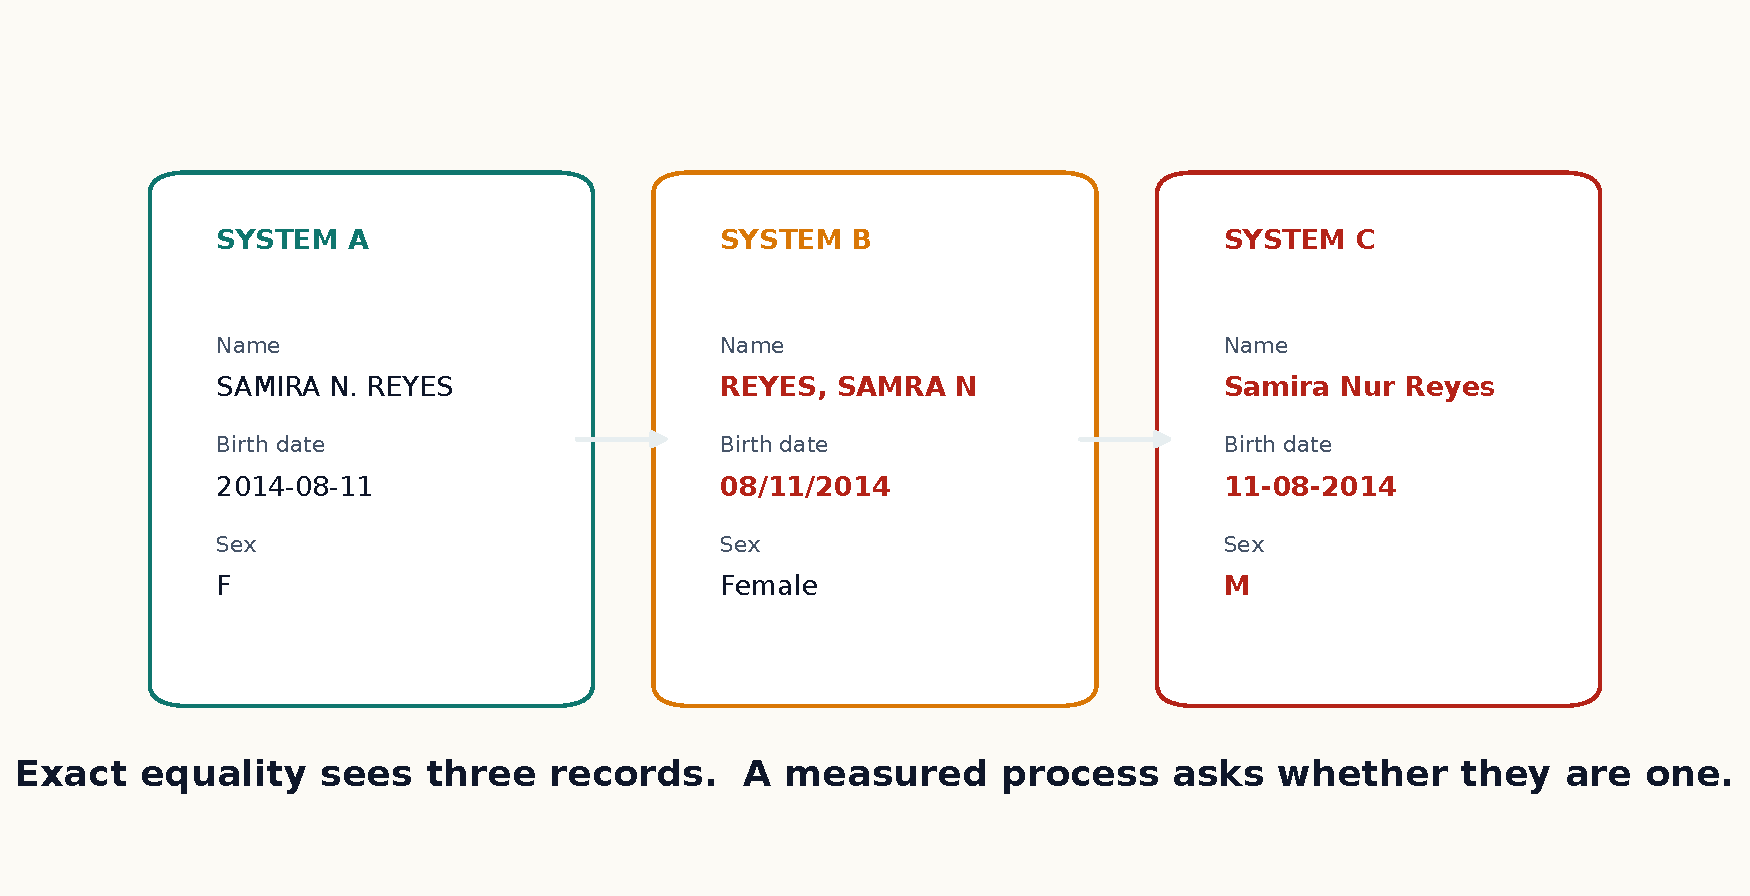
\includegraphics[width=0.81\linewidth]{figures/identity_variation.pdf}
\end{frame}

\begin{frame}{When records fail to connect, people disappear from the decision}
  \vspace{0.20cm}
  \begin{columns}[T,onlytextwidth]
    \begin{column}{0.31\textwidth}
      \ledgerbox{AuditRed}{01 · Missing}{The same person disappears between waves.}
    \end{column}
    \begin{column}{0.31\textwidth}
      \ledgerbox{EvidenceAmber}{02 · Duplicate}{One person is counted more than once.}
    \end{column}
    \begin{column}{0.31\textwidth}
      \ledgerbox{CivicBlue}{03 · Distort}{Rates and denominators quietly shift.}
    \end{column}
  \end{columns}

  \vspace{0.72cm}
  \centering
  {\fontsize{25}{30}\selectfont\bfseries\color{MidnightInk}
  The interface can be correct while the identity layer is wrong.}

  \source{General problem class: operational databases with no shared, reliable identifier.}
\end{frame}

\begin{frame}{A hidden answer key turns trust into something measurable}
  \begin{columns}[T,onlytextwidth]
    \begin{column}{0.56\textwidth}
      \vspace{0.2cm}
      {\fontsize{21}{26}\selectfont\bfseries A synthetic world creates both the mess and the truth.}\par
      \vspace{0.30cm}
      {\fontsize{15}{19}\selectfont\color{Slate}
      The generator creates spelling, date, sex-code, and identifier errors—then keeps the answer key outside the pipeline.}
    \end{column}
    \begin{column}{0.40\textwidth}
      \vspace{0.12cm}
      \begin{tabular}{@{}lr@{}}
        \toprule
        \textbf{Stress test} & \textbf{Count} \\
        \midrule
        Name drift & \textcolor{AuditRed}{\textbf{396}} \\
        Birth-date drift & \textcolor{AuditRed}{\textbf{132}} \\
        Sex inconsistency & \textcolor{AuditRed}{\textbf{70}} \\
        Missing identifier & \textcolor{AuditRed}{\textbf{564}} \\
        \bottomrule
      \end{tabular}
    \end{column}
  \end{columns}
  \source{Fixed-seed synthetic generator; truth artifacts remain outside the lakehouse boundary.}
\end{frame}

\begin{frame}{A trustworthy pipeline is a sequence of evidence gates}
  \centering
  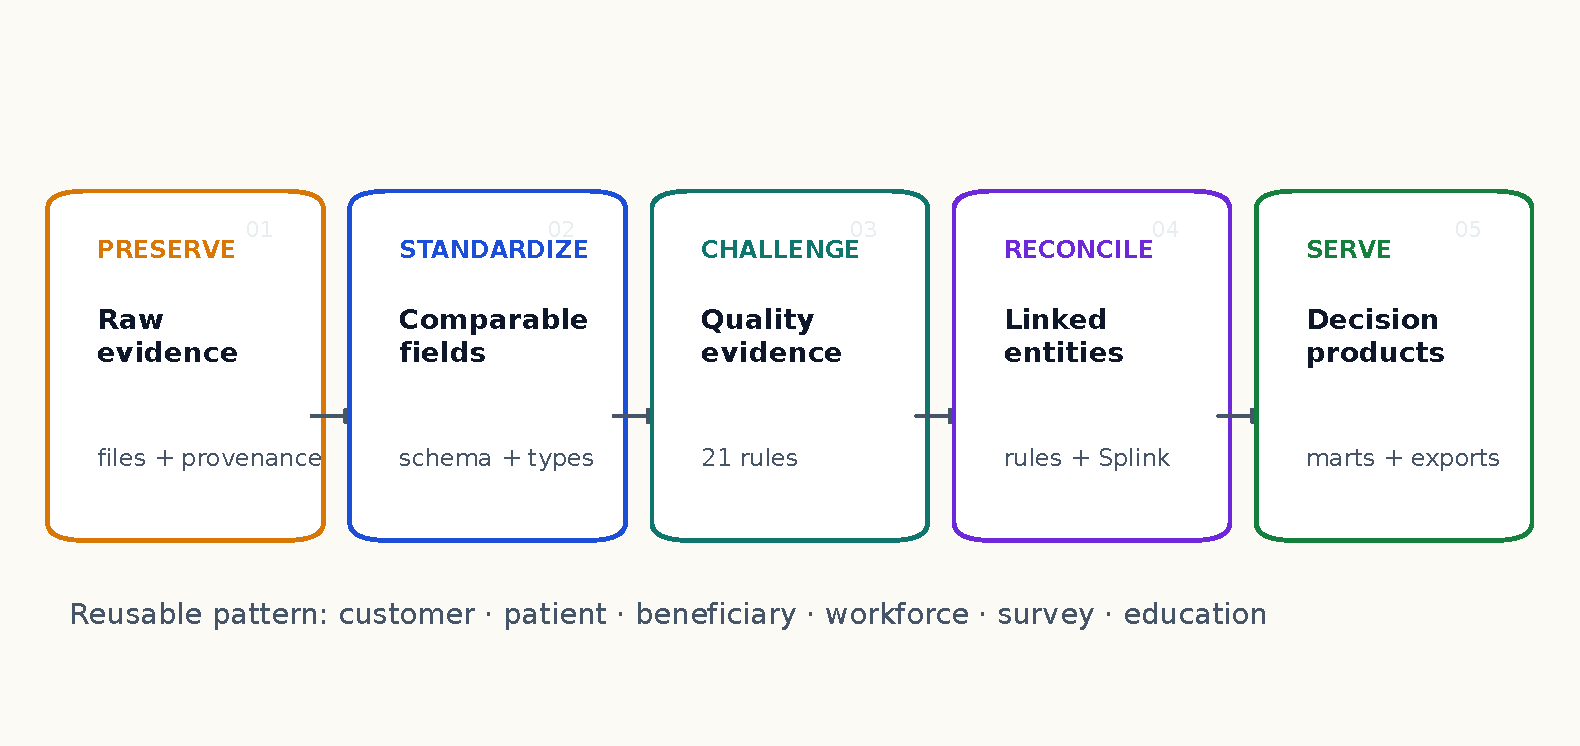
\includegraphics[width=0.87\linewidth]{figures/trust_pipeline.pdf}
\end{frame}

\begin{frame}{Quality checks caught 9 in 10 failures before they reached a decision}
  \centering
  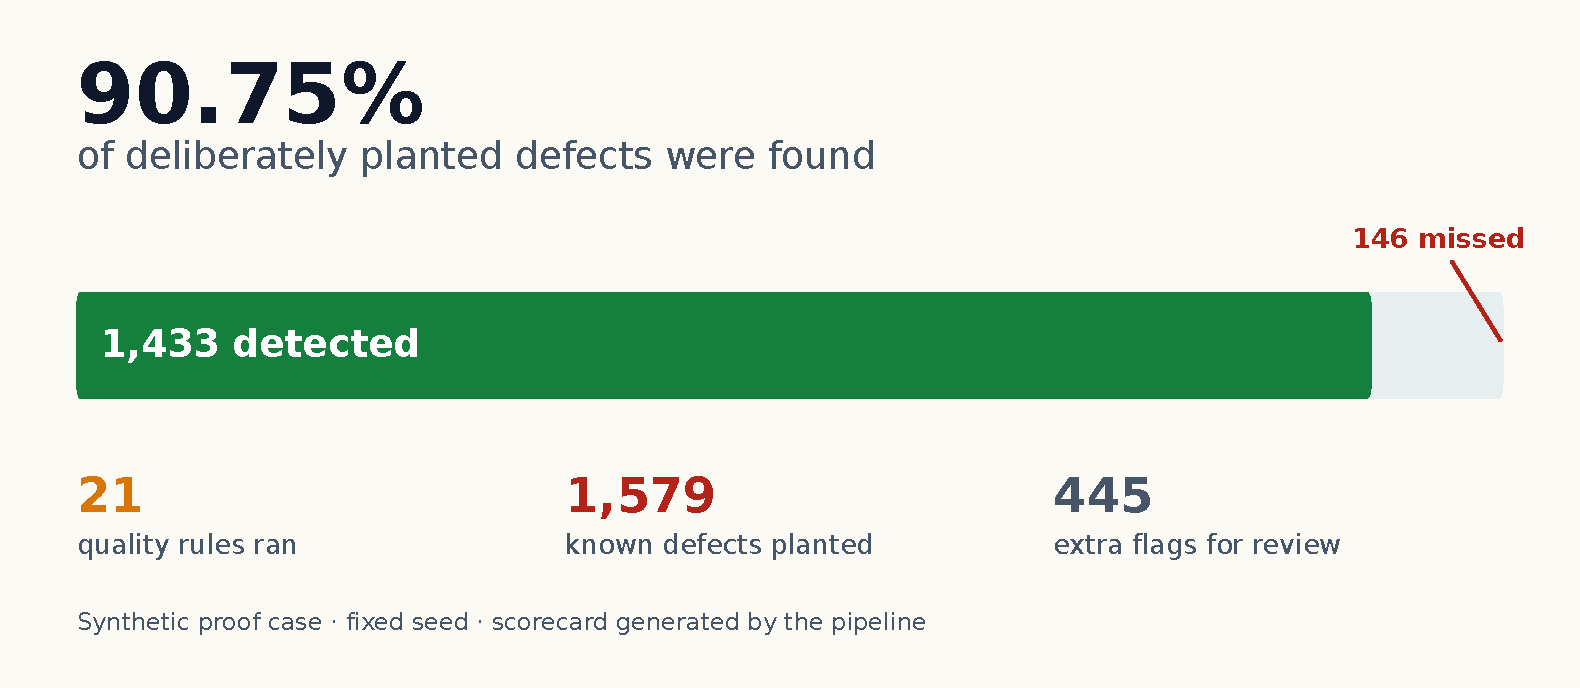
\includegraphics[width=0.94\linewidth]{figures/quality_detection.pdf}
\end{frame}

\begin{frame}{When a record is challenged, reviewers can see exactly why}
  \vspace{0.15cm}
  \begin{columns}[T,onlytextwidth]
    \begin{column}{0.48\textwidth}
      \ledgerbox{SignalTeal}{Where}{source file + row + field}
      \vspace{0.20cm}

      \ledgerbox{EvidenceAmber}{What}{rule + severity + observed value}
    \end{column}
    \begin{column}{0.48\textwidth}
      \ledgerbox{CivicBlue}{When}{pipeline run + reporting period}
      \vspace{0.20cm}

      \ledgerbox{ResolverViolet}{Then}{issue registry + review path}
    \end{column}
  \end{columns}
\end{frame}

\begin{frame}{Exact matching left 324 of 880 known relationships unresolved}
  \begin{columns}[c,onlytextwidth]
    \begin{column}{0.38\textwidth}
      \bigmetric{Slate}{63.2\%}\par
      {\fontsize{18}{22}\selectfont\bfseries recall}\par
      \vspace{0.22cm}
      {\fontsize{14}{18}\selectfont\color{Slate}The share of known relationships recovered: 556 of 880 using exact equality alone.}
    \end{column}
    \begin{column}{0.57\textwidth}
      {\fontsize{18}{23}\selectfont\bfseries Exact equality breaks when:}\par
      \vspace{0.25cm}
      {\fontsize{16}{21}\selectfont
      \textcolor{AuditRed}{\textbf{Names drift}}\par
      \textcolor{EvidenceAmber}{\textbf{Dates wobble}}\par
      \textcolor{CivicBlue}{\textbf{Codes disagree}}\par
      \vspace{0.42cm}
      \color{Slate}Precision alone cannot tell us who vanished from the join.}
    \end{column}
  \end{columns}
  \source{Deterministic baseline: 100.0\% precision, 63.2\% recall, 77.4\% F1.}
\end{frame}

\begin{frame}{Splink learns how much each imperfect clue should count}
  \vspace{0.18cm}
  \begin{columns}[c,onlytextwidth]
    \begin{column}{0.22\textwidth}
      \ledgerbox{ResolverViolet}{Name}{similarity, not equality}
    \end{column}
    \begin{column}{0.05\textwidth}
      \centering\fontsize{24}{24}\selectfont\color{Slate}+
    \end{column}
    \begin{column}{0.22\textwidth}
      \ledgerbox{ResolverViolet}{Date}{calendar-aware distance}
    \end{column}
    \begin{column}{0.05\textwidth}
      \centering\fontsize{24}{24}\selectfont\color{Slate}+
    \end{column}
    \begin{column}{0.22\textwidth}
      \ledgerbox{ResolverViolet}{Identity}{source ID + sex + source group}
    \end{column}
    \begin{column}{0.05\textwidth}
      \centering\fontsize{24}{24}\selectfont\bfseries\color{Slate}>
    \end{column}
    \begin{column}{0.13\textwidth}
      \centering
      \bigmetric{ResolverViolet}{p}\par
      {\fontsize{11}{13}\selectfont match probability}
    \end{column}
  \end{columns}

  \vspace{0.65cm}
  \centering
  {\fontsize{16}{20}\selectfont\bfseries Exact and fuzzy evidence belong inside one trained model.}\par
  {\fontsize{12}{16}\selectfont\color{Slate}Method: probabilistic entity resolution using a Fellegi--Sunter model.}
\end{frame}

\begin{frame}{One model is trained, saved, and reloaded for inference}
  \centering
  % Coordinate map:
  % (population) at (0,0) — 3.45cm x 1.65cm — all baseline/endline records
  % (model) at (4.35,0) — 3.45cm x 1.65cm — train and persist model JSON
  % (inference) at (8.70,0) — 3.45cm x 1.65cm — fresh linker loads and predicts
  % Arrows: population -> model and model -> inference, no edge labels.
  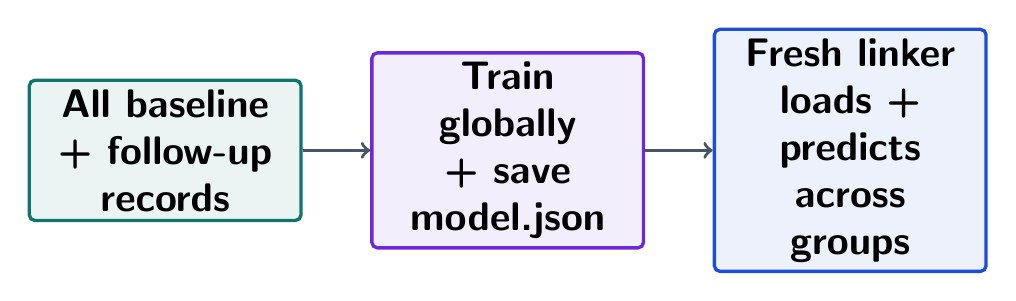
\begin{tikzpicture}[x=1cm,y=1cm]
    \node[draw=SignalTeal,very thick,fill=SignalTeal!8,rounded corners=2pt,
          minimum width=3.45cm,minimum height=1.65cm,text width=3.05cm,
          align=center,font=\fontsize{14}{17}\selectfont\bfseries] (population) at (0,0)
          {All baseline + follow-up records};
    \node[draw=ResolverViolet,very thick,fill=ResolverViolet!8,rounded corners=2pt,
          minimum width=3.45cm,minimum height=1.65cm,text width=3.05cm,
          align=center,font=\fontsize{14}{17}\selectfont\bfseries] (model) at (4.35,0)
          {Train globally + save model.json};
    \node[draw=CivicBlue,very thick,fill=CivicBlue!8,rounded corners=2pt,
          minimum width=3.45cm,minimum height=1.65cm,text width=3.05cm,
          align=center,font=\fontsize{14}{17}\selectfont\bfseries] (inference) at (8.70,0)
          {Fresh linker loads + predicts across groups};
    \draw[->,very thick,color=Slate] (population.east) -- (model.west);
    \draw[->,very thick,color=Slate] (model.east) -- (inference.west);
  \end{tikzpicture}

  \vspace{0.35cm}
  {\fontsize{16}{20}\selectfont\bfseries The weights on exact and fuzzy evidence are learned once; production links come only from the loaded model.}
  \source{Config: configs/linkage\_rules.yml · Runner: scripts/run\_linkage\_example.py}
\end{frame}

\begin{frame}{Splink raised true links from 556 to 812}
  \centering
  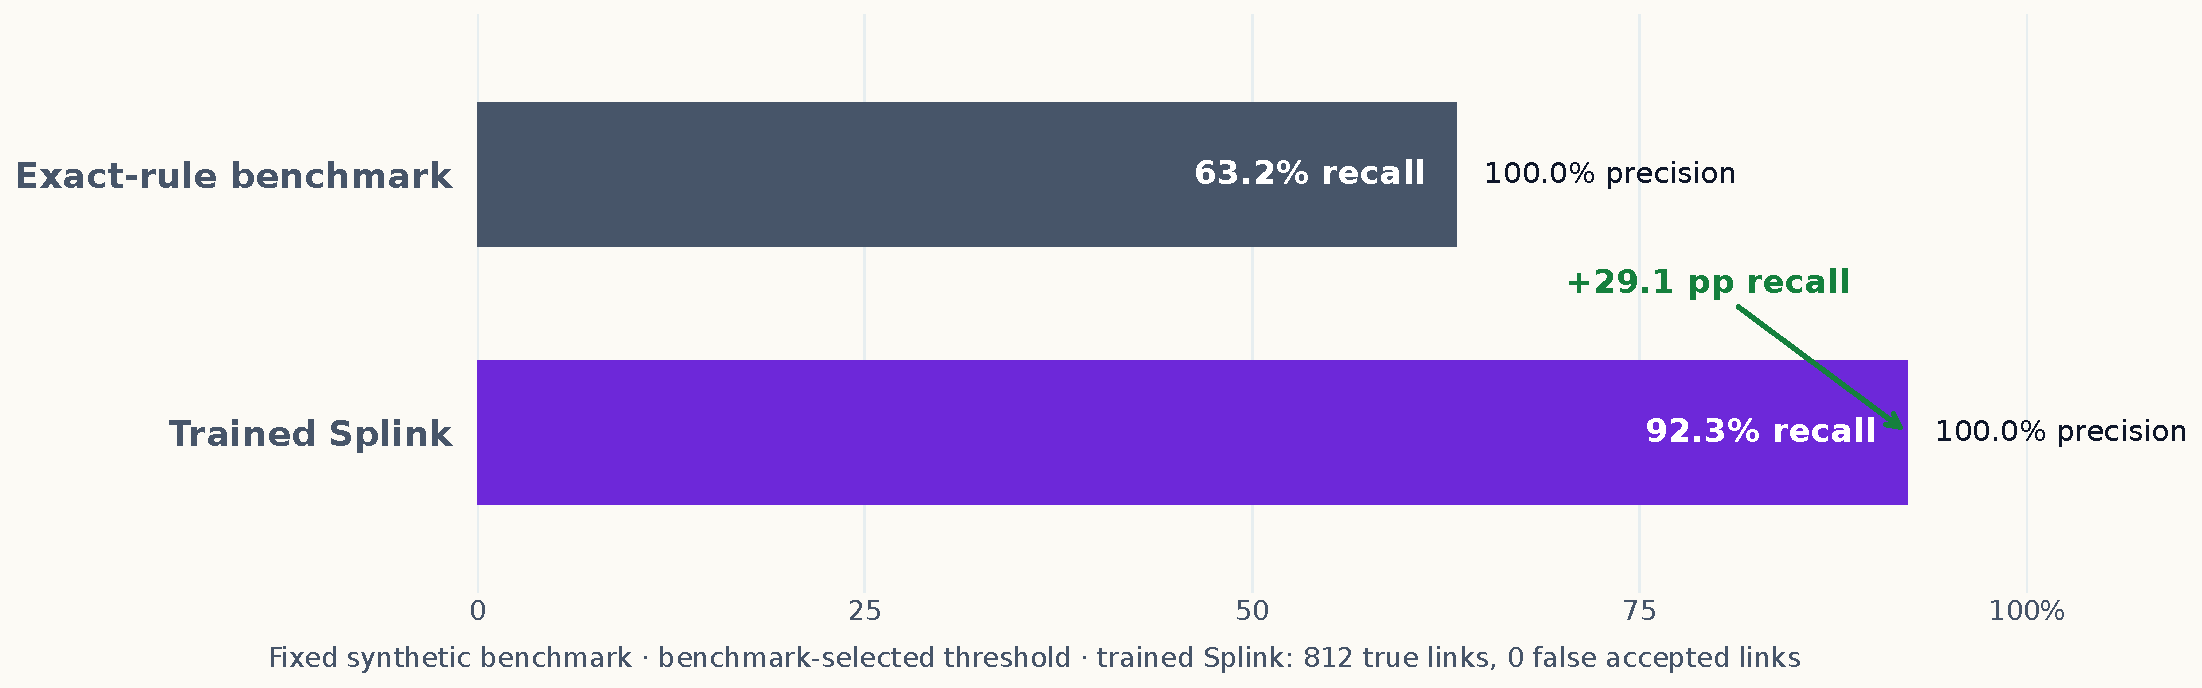
\includegraphics[width=0.97\linewidth]{figures/linkage_comparison.pdf}
\end{frame}

\begin{frame}{Even global Splink misses 7 of 26 cross-group moves}
  \begin{columns}[T,onlytextwidth]
    \begin{column}{0.48\textwidth}
      \eyebrow{What this proves}
      \par
      \vspace{0.12cm}
      {\fontsize{14}{19}\selectfont
      \textbf{The full pipeline runs.}\par\vspace{0.08cm}
      \textbf{Scorecards use known truth.}\par\vspace{0.08cm}
      \textbf{Trained Splink reaches 92.3\% recall with 0 false accepted links.}}
    \end{column}
    \begin{column}{0.48\textwidth}
      \eyebrow{What production must still prove}
      \par
      \vspace{0.12cm}
      {\fontsize{14}{19}\selectfont
      \textbf{Synthetic difficulty is not field prevalence.}\par\vspace{0.08cm}
      \textbf{Seven of 26 cross-group moves remain unresolved.}\par\vspace{0.08cm}
      \textbf{Thresholds need governance and review.}}
    \end{column}
  \end{columns}

  \vspace{0.10cm}
  \colorbox{EvidenceAmber!12}{\parbox{0.94\linewidth}{\centering\fontsize{13}{17}\selectfont\bfseries Cross-group transfer recall rose from 26.9\% to 73.1\%—and the remaining gap stays visible.}}
\end{frame}

\begin{frame}{Where databases disagree, the same trust layer can travel}
  \vspace{0.12cm}
  \begin{columns}[T,onlytextwidth]
    \begin{column}{0.31\textwidth}
      \ledgerbox{SignalTeal}{Customer}{CRM + billing + support}
      \vspace{0.16cm}
      \ledgerbox{CivicBlue}{Patient}{clinic + lab + claims}
    \end{column}
    \begin{column}{0.31\textwidth}
      \ledgerbox{EvidenceAmber}{Beneficiary}{intake + delivery + survey}
      \vspace{0.16cm}
      \ledgerbox{ResolverViolet}{Workforce}{HR + payroll + training}
    \end{column}
    \begin{column}{0.31\textwidth}
      \ledgerbox{VerifiedGreen}{Research}{panel + registry + follow-up}
      \vspace{0.16cm}
      \ledgerbox{Slate}{Education}{enrollment + program + outcomes}
    \end{column}
  \end{columns}
  \source{The product is not another database; it is evidence about which connections deserve trust.}
\end{frame}

\begin{frame}{The repository carries an evidence ledger—not a promise}
  \centering
  \vspace{0.10cm}
  {\fontsize{14.4}{17}\selectfont
  \begin{tabular}{@{}p{0.46\linewidth}p{0.46\linewidth}@{}}
\toprule
Assurance & Repository evidence \\
\midrule
\textbf{Regression protection} & \textcolor{SignalTeal}{\textbf{407}} automated tests \\
\textbf{Model contracts} & \textcolor{SignalTeal}{\textbf{27}} warehouse tests \\
\textbf{Known-failure monitoring} & \textcolor{SignalTeal}{\textbf{21}} quality rules \\
\textbf{End-to-end dependencies} & \textcolor{SignalTeal}{\textbf{8}} orchestrated assets \\
\textbf{Decision-ready outputs} & \textcolor{SignalTeal}{\textbf{6}} audience views \\
\textbf{Synthetic-only boundary} & \textcolor{SignalTeal}{\textbf{PASS}} privacy scan \\
\bottomrule
\end{tabular}
}
  \source{Counts generated from repository artifacts at build time; privacy status reflects the synthetic-only release.}
\end{frame}

\begin{frame}[plain]
  \vspace{0.84cm}
  \eyebrow{Measured Trust}
  \vfill
  {\fontsize{33}{39}\selectfont\bfseries\color{MidnightInk}
  A trustworthy pipeline does not merely move data—}

  \vspace{0.18cm}
  {\fontsize{33}{39}\selectfont\bfseries\color{SignalTeal}
  it measures what survives the journey.}
  \vfill
  {\fontsize{12}{15}\selectfont\color{Slate}
  Synthetic school-feeding proof case · reusable architecture for disconnected relational systems}
  \vspace{0.55cm}
\end{frame}

\end{document}
